
\documentclass[a4paper,11pt]{article}
\usepackage[polish]{babel}
\usepackage[OT4]{fontenc}
\usepackage[utf8]{inputenc}
\usepackage{graphicx}
\usepackage{subfig}
\usepackage{epstopdf}




\date{06/05/2014}


%opening
\title{PAMSI -- testowanie algorytmów wyszukiwania w grafie}
\author{Piotr Wilkosz}
\captionsetup{belowskip=12pt,aboveskip=4pt}
\begin{document}

\maketitle

\section{Wstęp}
Celem ćwiczenia było przetestowanie implementacji algorytmów wyszukiwania ścieżki w grafie. Graf został stworzony 
na podstawie listy incydencji. Przetestowano następujące algorytmy:
  \begin{itemize}
   \item Przeszukiwanie wgłąb - DFS
   \item Przeszukiwanie wszerz - BFS
   \item Przeszukiwanie grafu poczynając od najkrótszej ścieżki - Best - First Search
  \end{itemize}
Zadaniem było zmierzenie czasu wykonywania operacji wyszukania losowego elementu w grafie.
\section{Wyniki pomiarów}
\begin{enumerate}
 \item DFS
   
  \begin{table}[th]
  \centering
    \caption{Pomiar czasu przeszukiwania wgłąb w grafie}

      \begin{tabular}{|l|l|l|}
	\hline
	N & czas & odchylenie \\
    \hline
  10 & 0.000241798 & 0.000197743 \\
  \hline
100 & 0.00295474 & 0.00432009 \\
\hline
1000 & 0.126165 & 0.334439 \\
\hline
10000 & 0.56064 & 1.12066 \\
\hline
50000 & 3.74226 & 11.2241 \\
\hline
100000 & 9.42976 & 19.3432 \\
\hline
    \end{tabular}
    \end{table}
    \newpage
 \begin{figure}[th]
\centering
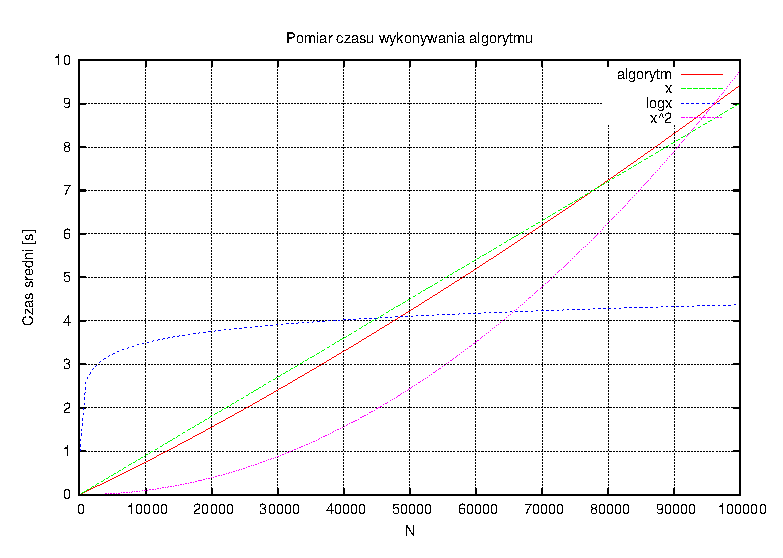
\includegraphics[width=0.8\textwidth]{../prj/wykres13.eps}
\caption{Wykres do tabeli nr 1}
\label{Wykres do tabeli nr 1}
\end{figure} 
Na podstawie wykresu czas operacji przeszukiwania wgłąb szacuje się jako liniowy. Duże odchylenie od średniego czasu przeszukiwania świadczy o tym,
 iż zarówno przypadek pesymistyczny, jak i optymistyczny przypada z jendakowym prawdopodbieństwem, co powoduje znaczące zróżnicowanie.
\item BFS
  \begin{table}[th]
  \centering
  
    \caption{Pomiar czasu przeszukiwania wszerz w grafie}

      \begin{tabular}{|l|l|l|}
	\hline
	N & czas & odchylenie \\
    \hline
10 & 4.5747e-06 & 1.52169e-06 \\
\hline
100 & 0.00106285 & 0.00193947 \\
\hline
1000 & 0.0216128 & 0.0473675 \\
\hline
10000 & 0.339568 & 0.941901 \\
\hline
50000 & 1.76083 & 5.35834 \\
\hline
100000 & 10.5094 & 39.9244 \\
\hline
    \end{tabular}
    \end{table}
    \newpage
\begin{figure}[th]
\centering
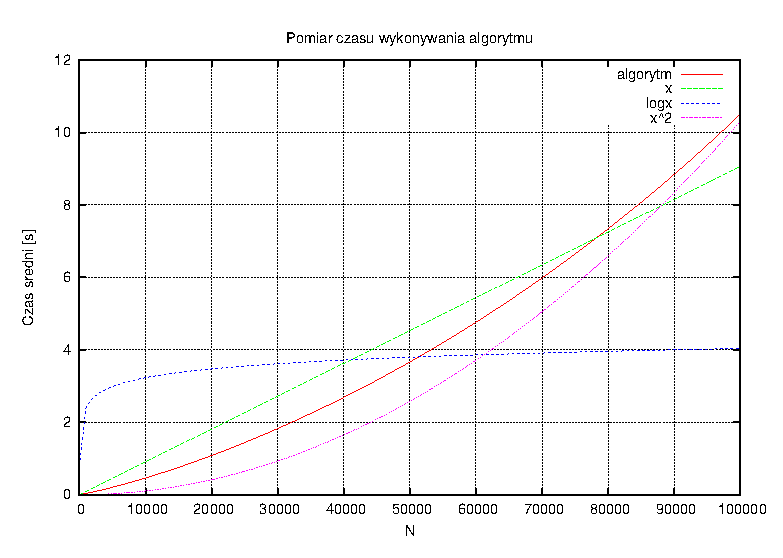
\includegraphics[width=0.8\textwidth]{../prj/wykres14.eps}
\caption{Wykres do tabeli nr 2}
\label{Wykres do tabeli nr 2}
\end{figure} 
Na podstawie wykresu czas operacji przeszukiwania wszerz szacuje się jako liniowy. Podobnie jak w przypadku wcześniejszym, zaobserwować można 
spore odchylenie, jednak uśrednienie wyników daje czas proporcjonalny do sumy liczb wierzchołków i krawędzi w grafie.
\item Best - First Search

\begin{table}[th]
\centering
    \caption{Pomiar czasu przeszukiwania typu best - first w grafie}

      \begin{tabular}{|l|l|l|}
	\hline
	N & czas & odchylenie \\
    \hline
 10 & 0.000279491 & 0.000470026 \\
 \hline
100 & 0.00318932 & 0.00492697 \\
\hline
1000 & 0.0417995 & 0.0982492 \\
\hline
10000 & 0.70878 & 1.24863 \\
\hline
50000 & 4.73391 & 9.98982 \\
\hline
100000 & 11.1066 & 17.9514 \\
\hline
    \end{tabular}
    \end{table}
    \newpage

    \begin{figure}[th]
\centering
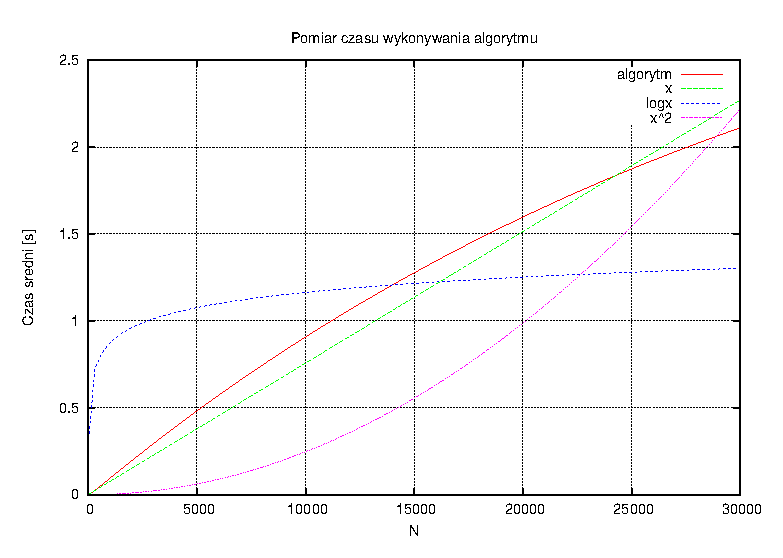
\includegraphics[width=0.8\textwidth]{../prj/wykres15.eps}
\caption{Wykres do tabeli nr 3}
\label{Wykres do tabeli nr 3}
\end{figure} 
Z powyższych danych mozna wyciągnąć podobne wnioski jak w przypadku dwóch poprzednich algorytmów. Czas wykonania operacji jest liniowy.
\end{enumerate}

\section{Wnioski}

\begin{itemize}
\item Wszystkie powyższe algorytmy osiągają podobną złożoność obliczeniową.

\item wykorzystanie uprzednio stworzonych struktur danych, jak np. tablica asocjacyjna, pozwoliło na bardziej intuicyjną implementację algorytmów.

\item Niestety badane algorytmy mogą okazać się mało efektywnym sposobem przeszukiwania grafów. Efekty ich działania są zbyt mocno zależne od struktury grafu. O efektywności
wykonania algorytmu w wielu sytuacjach decyduje losowe wybranie szukanego elementu, co często może prowadzić do sytuacji optymistycznej, ale także pesymistycznej.
\end{itemize}

\end{document}
